\documentclass[12pt]{report}
\usepackage{balance}			                    % proper column balancing 
\usepackage{cite}			                        % well-formed numeric citations
\usepackage{epsfig}			                        % add support for `EPS' figures
\usepackage{epstopdf}			                    % automatic `EPS' to `PDF' conversion
\usepackage[T1]{fontenc}		                    % enable `Type 1' fonts
\usepackage[pagebackref = false, pdftex]{hyperref}	% add support for hypertext marks
\usepackage{graphicx}			                    % add support for graphics
\usepackage{listings}			                    % add support for source code listings
\usepackage{mathptmx}			                    % use `Times' as the default font
\usepackage{subfigure}			                    % add support for `subfloats'
\usepackage{tikz}			                        % add support for custom graphics
\usetikzlibrary{calc} 
\usepackage{verbatim}	                            % better `verbatim'
\usepackage{xcolor}			                        % add support for color names
\usepackage{xspace}			                        % proper macro spacing
\usepackage{mdframed}
\usepackage{caption}
\usepackage{algorithm}
\usepackage{algorithmic}
\usepackage{minitoc}								% local table of content
\usepackage{geometry}
\geometry{
    a4paper,
    left = 3.5cm,
    top = 2.5cm,
    right = 2.5cm,
    bottom = 3.0cm
}

\usepackage{silence}

\WarningFilter{minitoc(hints)}{W0023}
\WarningFilter{minitoc(hints)}{W0028}
\WarningFilter{minitoc(hints)}{W0030}
\WarningFilter{minitoc(hints)}{W0099}
\WarningFilter{minitoc(hints)}{W0024}

\WarningFilter{blindtext}{} % this takes care of the `blindtext` messages

\usepackage[titletoc]{appendix}

% Font size and spacing of sections chapters
\usepackage{titlesec}
\titlespacing*{\chapter}{0pt}{0pt}{30pt}
\titleformat*{\section}{\large\bfseries} %14.4pt
\titleformat*{\subsection}{\normalsize\bfseries} %12pt
\titleformat{\chapter}[display]
{\normalfont%
    \LARGE %20.74pt
    \bfseries}{\chaptertitlename\ \thechapter}{20pt}{%
    \LARGE %20.74pt
}

% path of figures
\graphicspath{{./figures/} }

% name, title, keywords
\def\pname{webFuzz\xspace}
\def\ptitle{\pname: Implementation of a Grey-box Fuzzing Tool for Web Applications}
\def\pkeywords{keyword1, keyword2}

% comment out the following line to disable comments in text
% \newcommand{\commentsenabled}{X}
% comment commands
\ifdefined\commentsenabled
\newcommand{\el}[1]{\textbf{\color[rgb]{1,0,0} elathan: #1}}
\newcommand{\mac}[2]{\textbf{\color[rgb]{0,0,1} marcos: #1}}
\else
\newcommand{\el}[1]{}
\newcommand{\mac}[2]{}
\fi

% listings setup
\lstset{
	backgroundcolor	= \color{white},
	basicstyle	= \footnotesize, % \scriptsize
	breaklines	= true,
	captionpos	= b,
	commentstyle	= \color{gray}\ttfamily,
	frame		= lines, 
	language	= C++, 
	numbers		= left,
	tabsize		= 2,
	xleftmargin	= 6pt,
}

% hyperref setup
\hypersetup{
	unicode,
	citecolor	= black,
	colorlinks	= true,
	filecolor	= black,
	linkcolor	= black,
	pagebackref	= true,
	pdfkeywords	= {\pkeywords},
	pdftitle	= {\ptitle},
	urlcolor	= black,
} 

% checkmark
\def\checkmark{\tikz\fill[scale=0.4](0,.35) -- (.25,0) -- (1,.7) -- (.25,.15) -- cycle;} 

% hacks
\newenvironment{code}{\small\verbatim}{\endverbatim\normalsize}
\newcommand{\note}[1]{\noindent\textbf{\color{red}[#1]}}
\newcommand{\commentout}[1]{}

% custom macros
\newcommand{\ie}{\emph{i.e.,}\xspace}
\newcommand{\eg}{\emph{e.g.,}\xspace}
\newcommand{\etc}{\emph{etc.}\xspace}

\linespread{1.5} 
% \linespread{1.25} 

\begin{document}
\begin{titlepage}
\begin{center}
\vspace*{1cm}

\textcolor{black}{Thesis Dissertation}

\vspace*{2cm}

\textcolor{black}{\Large{\textbf{\MakeUppercase{\ptitle{}}}}}

\vspace*{2cm}

\textcolor{black}{\large{\textbf{Marcos Antonios Charalambous}}}

\vspace*{2cm}
\textcolor{black}{\Large{\textbf{\MakeUppercase{University of Cyprus}}}}

\vspace*{2cm}


\includegraphics[width=0.2\textwidth]{ucy-logo.png}

\vspace*{2cm}

\textcolor{black}{\Large{\textbf{\MakeUppercase{Computer Science Department}}}}

\vspace*{4cm}

\textcolor{black}{\normalsize{December 2020}}
\begin{tikzpicture}[remember picture, overlay]
  \draw[line width = 1pt] ($(current page.north west) + (1in,-1in)$) rectangle ($(current page.south east) + (-1in,1in)$);
\end{tikzpicture}
\end{center}
\end{titlepage}

\begin{titlepage}

\begin{center}
\LARGE{\textbf{\MakeUppercase{University of Cyprus}}}

\Large{\textbf{\MakeUppercase{Computer Science Department}}}

\vspace*{5cm}

\large{\textbf{\ptitle{}}}

\vspace*{0.5cm}

\large{\textbf{Marcos Antonios Charalambous}}

\vspace*{5cm}

\normalsize{Supervisor}

\normalsize{Dr. Elias Athanasopoulos}

\vspace*{3cm}

\normalsize{Thesis submitted in partial fulfilment of the requirements for the award of degree of Bachelor in Computer Science at University of Cyprus}

\vspace*{2cm}

\normalsize{December 2020}
\end{center}

\end{titlepage}

\pagenumbering{roman} % start roman page numbering

\setlength{\parindent}{0em}
\setlength{\parskip}{1.0em}

\section*{\LARGE{Acknowledgments}}

I would like to express sincere gratitude to my Thesis Supervising Professor Dr. Elias Athanasopoulos for his crucial guidance, encouragement, support and advice he provided to help me complete and accomplish this dissertation. During the past year, Dr. Athanasopoulos' interest, enthusiasm and expert knowledge in the field of Cybersecurity has undoubtedly been a source of inspiration to me. He sparked my interest in computer security which has led to this thesis. All his positive input made this endeavour an exciting experience. 

Also, I would like to thank my fellow students Demetris Kaizer and Orpheas Van Rooy for their excellent teamwork and participation in a greater project that combines each of our thesis.

Furthermore, I would like to thank PhD. candidate Michalis Papapevripides of SREC Lab for his timely response to any issues that arose and for the assistance he provided me in resolving them.

Moreover, I want to thank all my professors from whom I received invaluable knowledge enabling me to become a Computer Scientist after my four years of study at the Department of Computer Science of the University of Cyprus.

Finally, I would like to thank my family and friends for being with me during my trials and tribulations, supporting me at every step of the way.

\newpage

\section*{\LARGE{Abstract}}

Testing software is a common practice for exposing unknown vulnerabilities
in security-critical programs that can be exploited with malicious intent.
A bug-hunting method that has proven to be very effective is a technique
called fuzzing. 

Specifically, this type of software testing is frequently in the
form of fuzzing of native code, which includes subjecting the program to
enormous amounts of unexpected or malformed inputs in an automated fashion.

This is done to get a view of their overall robustness to detect and fix
critical bugs or possible security loopholes. For instance, a program crash
when processing a given input may be a signal of memory-corruption
vulnerability.

Although fuzzing has significantly evolved in analysing native code, web
applications, invariably, have received limited attention until now. 

This thesis explores the technique of gray-box fuzzing of web applications and the
construction of a fuzzing tool that automates the process of discovering
bugs in web applications. We design, implement and evaluate webFuzz, which is a prototype grey-box
fuzzer for web applications. 

WebFuzz leverages instrumentation for successfully
detecting reflective Cross-Site Scripting (XSS) vulnerabilities faster than other
black-box fuzzers. The functionality of webFuzz is demonstrated using web applications
written in PHP; namely WordPress and Drupal.

\dominitoc
\tableofcontents
\listoffigures
\listoftables

% outline
\chapter{Introduction}
\pagenumbering{arabic} % start arabic page numbering
\minitoc
\vspace*{1cm}

This the first and introductory chapter of this thesis. Here we analyse what motivated me to start this project, any related work regarding fuzzing, the contribution that our fuzzing tool has and the outline of the topics of the rest of the chapters included in this thesis.

% NEW SECTION
\section{Motivation}
Fuzzing is now recognised as an essential process for discovering hidden bugs in computer software. Automated software testing or fuzzing is a tried and tested method of generating or mutating inputs and passing them to programs in search of bugs. The spark in the fuzzing 'revolution' to discover bugs in software in an automated fashion has been precipitated with the introduction of AFL ~\cite{zalewski2015american}, a state-of-the-art fuzzer that produces feedback during fuzzing by leveraging instrumentation of the analysed program. By creating this \textit{feedback loop}, fuzzers can significantly improve their performance as they can determine whether an input is interesting, namely it triggers a new code path, and uses that input to produce other test cases.

Software testing plays a vital role in the software development cycle because when vulnerabilities are present, they can have severe and irreparable consequences. By exploiting software bugs, adversaries can perform data breaches, install malicious malware or even take complete control of a device. Detecting bugs before they get exploited is possible while also being a demanding task. Mainly because bugs are triggered when an unexpected input is given to the program, something which is difficult to fully simulate through statically written unit tests. This is because unit tests usually revolve around expected inputs in order to test the intended functionality of code ~\cite{aschermann2019nautilus}.

Although automated software testing has become an attractive field of research, it still has a long way to go, especially for web applications ~\cite{doupe2010johnny}. As the Internet infrastructure expands, more software written in native code is migrating to web applications. This attracts more malicious attacks on web applications. Hence, there is a strong need for the development of automated vulnerabilities scanners that target web applications.
 
% NEW SECTION REPHRASE
\section{Related Work}
 Numerous fuzzers recently developed try to optimize the fuzzing process by proposing various methodologies ~\cite{godefroid2012sage, stephens2016driller, rawat2017vuzzer, aschermann2019nautilus, aschermann2019redqueen, hoffman2020Was, osterlund2020parmesan }. For instance, most of the fuzzers take advantage of instrumentation on the source or binary level. That is, inserting code to the program in order to receive feedback when a code block gets
triggered and try to adjust the generated inputs to improve code coverage. Others utilize concolic/symbolic execution in order to extract useful information about the program and use that information for improving the input generation process ~\cite{stephens2016driller,godefroid2005dart,godefroid2012sage}. However, all these fuzzers are currently targeted towards finding vulnerabilities in native code, while web applications have received limited attention. More related work will be see again at Chapter ~\ref{relatedwork}.


\section{Contributions}
A highly automated testing technique that covers numerous boundary cases
using invalid data (from files, network protocols, API calls, and other targets)
as application input to better ensure the absence of exploitable vulnerabilities.
The name comes from modem applications’ tendency to fail due
to random input caused by line noise on fuzzy telephone lines.A highly automated testing technique that covers numerous boundary cases
using invalid data (from files, network protocols, API calls, and other targets)
as application input to better ensure the absence of exploitable vulnerabilities.
The name comes from modem applications’ tendency to fail due
to random input caused by line noise on fuzzy telephone lines.



mutation-based fuzzer, might actively see the code paths executed in the target and make adjustments accordingly, which is very smart. EFS and AFL do exactly this

even google is very active in the industry of fuzzers https://github.com/google/oss-fuzz, atheris


% NEW SECTION
\section{Contributions}

\section{Outline Contents}
\chapter{Background}
\label{sec:background}
\minitoc
\vspace*{1cm}

In this chapter, we provide background information giving a detailed understanding of several key points about this thesis. First, we define what a Cross-Site Scripting bug is in web applications by giving specific examples of how this vulnerability may occur. Then, we briefly discuss what fuzzing is and the various categories that constitute it, showing how \emph{instrumentation} helps when used during grey-box fuzzing. Towards the end, this chapter discusses the concept of concurrency in Python and concludes with the containerization of services using Docker.

\section{Web Application Bugs}
The internet has been growing exponentially since its commercial inception in 1969 with the creation of ARPANET. Although there are over 1 billion pages currently online, writing a web application secure from any vulnerability can be extremely difficult. Every significant web application, especially large-scale ones that are composed of thousands of Lines of Code (LoC), have dangerous bugs in them. Popular social-networking site Facebook had bugs in its 100 million LoC that resulted in 50 million users having their personal data exposed ~\cite{facebook_data_breach,facebook_loc}. Such problems are not exclusive to complex web applications. Even the simplest web-apps can be the root of irreparable damage when they are exploited by attackers with ulterior motives. 

In fact, web application vulnerabilities are among the most frequent vulnerabilities reported in the Common Vulnerabilities and Exposures database (CVE). According to CVE 2019 data, Denial of Service  (DoS) (19.2\%) is ranked second and Cross-Site Scripting (XSS) (12.5\%) is fourth among the top Cybersecurity vulnerabilities ~\cite{cve}.

The Open Web Application Security Project (OWASP) Top 10 represents a broad consensus on the most critical security risks to web applications ~\cite{owasp2017}. One of the most pressing security issues on the Internet, according to the OWASP list, is Cross-Site Scripting (ranked 7).

XSS flaws occur whenever an application includes untrusted data in its web page responses without validating or escaping them first. In other words, the web application accepts input from the user and then attempts to display it without filtering for HTML tags or script code, such as JavaScript. JavaScript is an essential part of web applications as it is used during both frontend and backend development with all major web browsers having a dedicated engine to execute {\tt .js} code. So, allowing such untrusted code to be executed can hijack the browser, deface the website, redirect the user to dangerous sites and many other attacks. Some XSS types include Reflected(Non-Persistent or Type II), Stored (Persistent or Type I) and DOM-based(Type-0).

Reflected XSS ~\cite{rxss_def} vulnerabilities arise when arbitrary data is copied from a request and echoed into the application's immediate response. By not filtering the data input, scripting language code included within a request can be executed, whatever its content. In the case of Stored XSS vulnerabilities, the malicious payload is permanently stored in storage such as a database residing on a server and is only later outputted by an unsuspecting query. Locations, where Stored XSS may occur, include Web forums or blog comments. 

\pname{} focuses on detecting bugs that can lead to both Reflected or Stored Cross-Site Scripting, that are among the most common of XSS attacks. A step-by-step illustration of the latter can be seen in Figure ~\ref{fig:storedxss} and the former in Figure ~\ref{fig:reflectedxss}. In both illustrations, the attacker and victim are represented by \pname{}.

It is imperative that we understand what an RXSS (Reflected XSS) bug typically looks like, in order to grasp the thesis' perspective on such vulnerabilities. Usually, RXSS is caused due to a failure to sanitise user input. For instance, let us assume that we have a simple login page with two input fields: the username and password. The login page also displays the appropriate error messages back to the user if the login fails. An implementation of this in PHP could look something like Listing ~\ref{lst:vuln_login_sub}.

\begin{lstlisting}[aboveskip=\baselineskip, showstringspaces=false, frame=single, language=PHP, caption={\textit{Vulnerable login form}}, numberstyle=\color{gray}, numbersep=5pt, label={lst:vuln_login_sub}]
<?php
$username=$_POST['username'];
$pwd=$_POST['password'];
if (search_username($username)) {
   if (match_username_password($username, $pwd)) {
      // do normal login procedures
   } else {
      echo 'Wrong Password';
   }
} else {
      echo 'Error' . $username . 'was not found.';
}
?>
\end{lstlisting}

\begin{figure}[ht]
 \centering
 \captionsetup{justification=centering}
 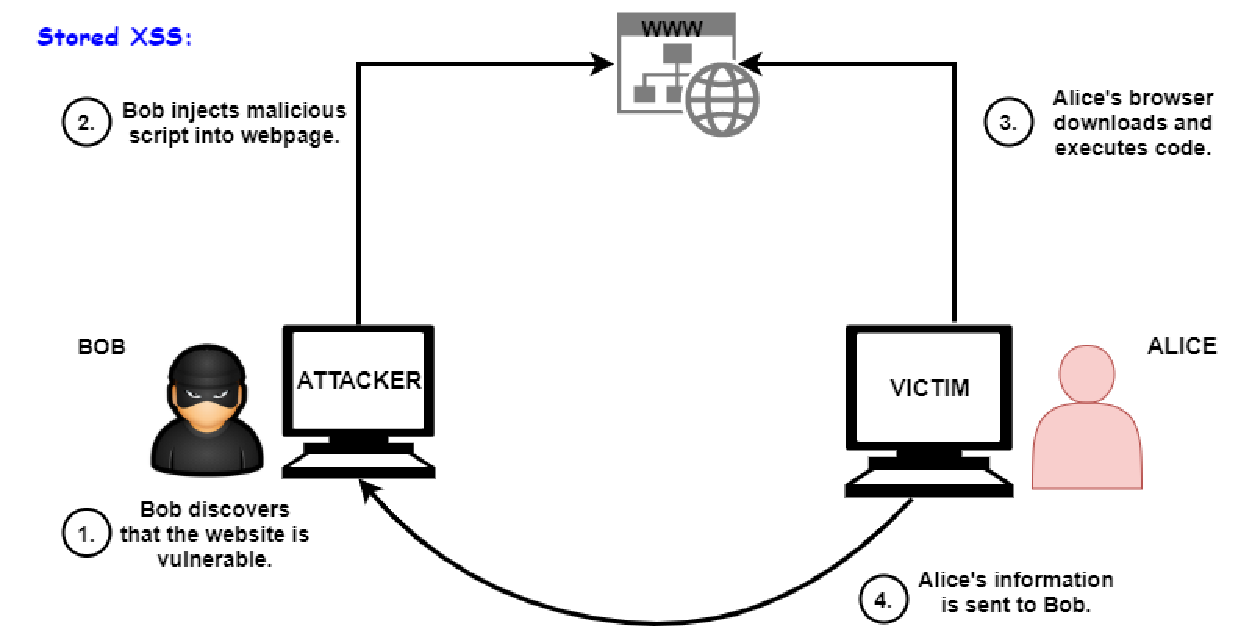
\includegraphics[width=\linewidth]{figures/storedxss.pdf}
 \caption[How Stored Cross-Site Scripting can be exploited by an attacker]{\textit{How Stored Cross-Site Scripting can be exploited by an attacker}}
 \label{fig:storedxss}
\end{figure}

\begin{figure}[ht]
 \centering
 \captionsetup{justification=centering}
 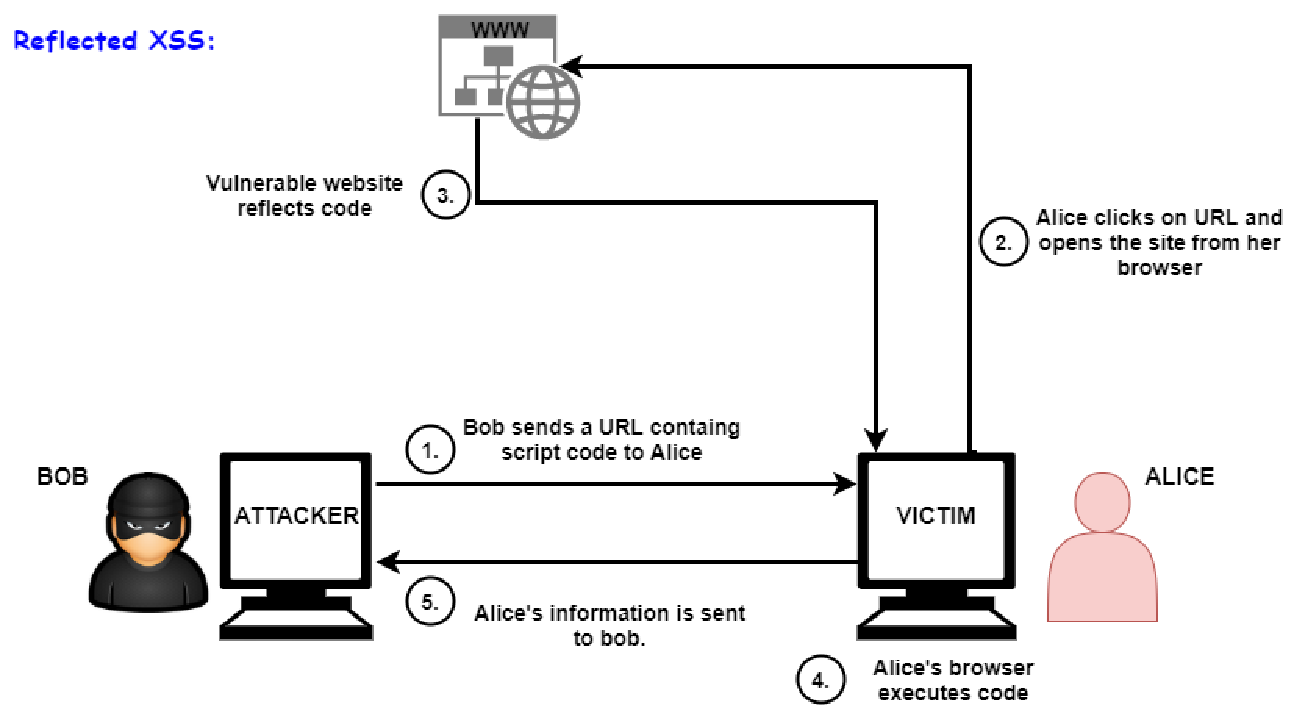
\includegraphics[width=\linewidth]{figures/reflectedxss.pdf}
 \caption[How Reflected Cross-Site Scripting can be exploited by an attacker]{\textit{How Reflected Cross-Site Scripting can be exploited by an attacker}}
 \label{fig:reflectedxss}
\end{figure}

The above code is faulty for two reasons. First, knowing a username exists offers clues for an attacker to guess a set of correct credentials much faster since only the password is left to find. But this design choice is not linked with Cross-Site Scripting. The source of the bug is on line 11 where the error message "{\tt the \$username was not found}" is displayed. Because {\tt \$username} is a variable that has not been sanitized, an attacker can inject malicious payload in this field that will be interpreted by the HTML parser according to whatever its content is. 

{\tt Exploit:} A victim is tricked into submitting a {\tt form} located in an attacker-controlled website. The malicious payload is designed to trigger the vulnerability found in the above login {\tt form} (Listing ~\ref{lst:vuln_login_sub}). As soon as the {\tt form} is submitted, the vulnerable login page is opened with the XSS script executed in it. When the victim tries to login, the XSS script can easily send the credentials to the attacker as well. 

Defeating XSS attacks is not dissimilar to defending against other types of code injection.
The input must be sanitized. User input containing HTTP code must be escaped or encoded to avoid its execution. System-wide measures such as Content Security Policy (CSP) ~\cite{csp_def} may be enabled to eliminate or mitigate XSS attacks. Nevertheless, flaws such as Buffer Overflows (CVE ranked 3 ~\cite{cve}) or Cross-Site Scripting issues comprise a majority of security incidents that malicious hackers exploit daily. 

\section{Fuzzing}
A promising method for discovering unknown vulnerabilities in programs and web applications proven to be very effective, is a technique called fuzzing (or fuzz testing) ~\cite{fuzzing_def}. Fuzzing was invented by Barton Miller at the University of Wisconsin, as one of several tools to test UNIX utilities ~\cite{mller1990fuzz}. With this quality assurance technique, the software is exercised using a vast number of anomalous inputs for inferring if any of them introduce security-related side-effects. A fuzzer, the tool that automates the aforementioned stress-testing process can be categorized in relation to its awareness of the program structure as black-, white-, or grey-box ~\cite{fuzzing_book}. 

A black-box fuzzer treats the program as a 'black box' and is unaware of internal structures. It conducts its test on the target through external interfaces and produces random inputs using no information about the target's underlying structure. More often than not, black-box fuzzers are only able to scratch the surface and expose "shallow" bugs ~\cite{fuzzing_owasp}. For example, the branch of the conditional statement "{\tt if x==5:}" has only one in $2\textsuperscript{32}$ chance of being executed if {\tt x} is a randomly chosen 32-bit input value (\ie an integer). That intuitively explains why black-box testing usually provides low code coverage and is unable to find bugs nestled deep in the program ~\cite{Godefroid2008AutomatedWF}.

A white-box fuzzer infers source code knowledge, such as source code auditing, to reveal
flaws in the software. It leverages program analysis to systematically
increase code coverage or to reach certain critical program locations otherwise unreachable. Program analysis can be based on either static or dynamic analysis, or their combination ~\cite{program_analysis_book}. They may also leverage symbolic execution to derive what inputs cause each part of a program to execute ~\cite{king1976symoblic}. It makes them effective at exposing bugs that hide deep in the program. By studying the application code, you can detect optional or proprietary features, which should be tested as well.

A fuzzer is considered grey-box when it leverages \emph{instrumentation} rather than program analysis to glean information about the coverage of a generated input from the program it tries to fuzz ~\cite{zalewski2015american,efs2007}. Adopting this process significantly reduces the 'guesswork' that occupies black-box fuzzers. This thesis explores in detail grey-box fuzzing, which combines elements of the white-box and black-box approaches since it uses the internals of the software, to a minimal extent, to help generate better test cases without needing full access to the code. 

We also explored the feasibility of constructing a fuzzing tool that will automate the process of discovering bugs in web applications. This was done by providing randomized invalid inputs to an under-analysis instrumented web application, mutating these inputs according to the feedback received and finding test cases that cause a systems crash or make them act inappropriately to prevent exploitable vulnerabilities.

\section{Instrumentation}
Typically, a fuzzer is considered more effective if it achieves a higher degree of code coverage. To be able to trigger any given bug, the fuzzer must first execute the code where the bug lies. So, widening code coverage increases the chances of executing unsafe pieces of code where bugs may reside. As mentioned in the previous section, using \emph{instrumentation} may be the key to achieving a higher code-coverage percentage. 

However, some studies have failed to reach a consensus on the correlation between code coverage and the number of bugs found ~\cite{klees2018Evaluation,coverage2014effectiveness}. 
Increasing global code coverage may be less effective in finding new bugs than, for instance, focusing on widening code coverage in targeted error-prone code areas as AFLGo ~\cite{bohme2017directed} does. Therefore, code coverage should be considered a secondary metric and the number of bugs found as the primary ~\cite{klees2018Evaluation}. Nevertheless, measuring coverage is crucial for any fuzzer.

Available fuzzers for web applications act in a black-box fashion~\cite{doupe2010johnny}; by applying brute force to the target with URLs that embed known web-attack payloads with little or no information about the underlying structure of the target. In contrast, \pname firstly instruments a web application by adding code that tracks all control flows triggered by an input and notifies the fuzzer, accordingly. Notifications can be embedded in the web application's HTTP response using custom headers or it can be outputted to a shared file or memory region. 

Consequently, the fuzzer sends requests to the target and analyses the responses to detect any requests of interest that would later help to improve the code coverage and as a result, trigger vulnerabilities nested deep in the web application's code. To measure code coverage we calculate the ratio of how many basic blocks were visited in respect to the total number of basic blocks instrumented. It gives us a good idea of the coverage but omits information such as sequences of basic blocks that were visited.

We instrumented web applications for delivering feedback once being fuzzed. As opposed to native applications, where several options exist for instrumenting their source or binary representation. We decided to instrument web applications by modifying the AST of PHP files and then reverting it to source code form. This provided us with crucial feedback on the basic blocks that are visited during the analysis. \emph{Instrumentation} performed by \pname on our targeted web application is similar to how AFL instruments binaries, but adapted to work in web applications.

\section{Concurrency}
Concurrency is defined as working on multiple tasks at the same time ~\cite{concurrency_realpython}. However, in Python this does not mean that they work in parallel, since only one core of the CPU is active at any given time. Instead, each task takes turns in occupying the core and executing their code. When a task is interrupted, its state is stored so it can restart from the point where it left off. 

Concurrency aims to speed up the overall performance of input/output (I/O) bound programs, whose performance can be slowed dramatically when they are obliged to frequently wait for I/O operation from an external resource. An example of such resources are requests over the internet or any type of network traffic that takes several orders of magnitude longer than CPU instructions. An illustration of the above can be seen in Figure ~\ref{fig:concurrency_example}:

\begin{figure}[ht]
 \centering
 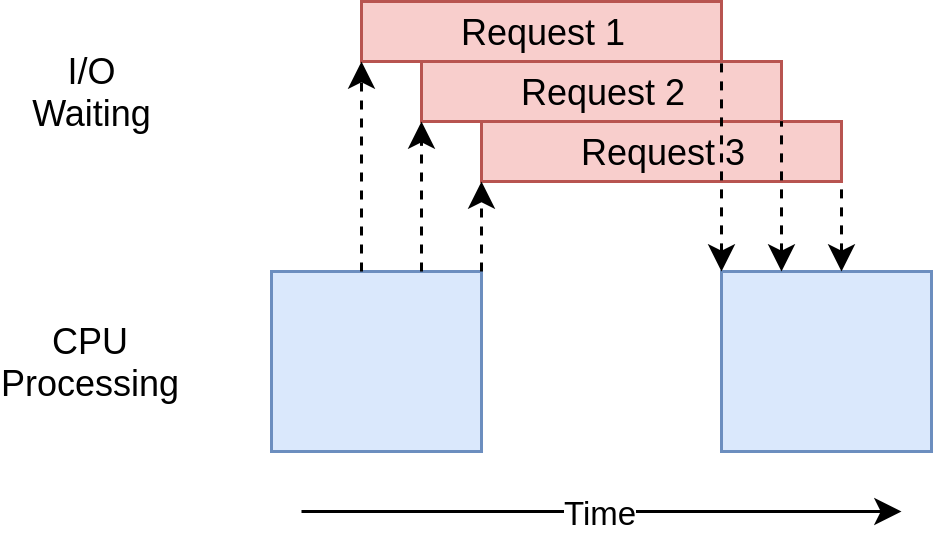
\includegraphics[width=\linewidth]{figures/concurrency_example.png}
 \caption[Requests over the internet processed concurrently]{\textit{Requests over the internet processed concurrently} ~\cite{concurrency_realpython}}
 \label{fig:concurrency_example}
\end{figure}

In Python, concurrency is expressed either through the Threading or AsyncIO (short for Asynchronous Input Output) ~\cite{asyncio} modules. Due to the infamous \emph{Global Interpreter Lock} (GIL) ~\cite{gil_realpython} Python has, both AsyncIO and Threading, they are single-threaded, single-process design. There was no clear advantage in using the latter so, AsyncIO was opted for instead, although initial work was done with {\tt threading} it was shelved. Not to mention the added complexity of using threads and making the program thread-safe. 

Briefly, GIL ensures there is only one thread running at any given time, thus making the use of multiple cores/processors with threads infeasible. In the Python community there is a general rule of thumb when it comes to I/O-bound problems; "Use asyncio when you can, threading when you must". More information on the AsyncIO module and its use in the \pname implementation can be found in Chapter ~\ref{sec:implementation}.

\section{Docker}
Docker containers ~\cite{docker_containers} provide developers the commodity for creating software locally with the knowledge that it will run identically regardless of the host environment ~\cite{using_docker_book}. Containers are an encapsulation of an application's dependencies that share resources with the host OS, unlike frequently used \emph{Virtual Machines}. During the evaluation, detailed in Chapter ~\ref{sec:evaluation}, a docker-compose {\tt YAML} file was created to allow multiple containers to be initiated and managed at the same time with a set of pre-defined configurations. 

Services are deployed with containers through the use of Docker images. A Docker image consists of a collection of files that bundle together all the essentials, such as installations, application code and dependencies required to configure a fully operational container environment. Official Docker images can be found at Docker Hub ~\cite{docker_hub}.
\chapter{Architecture}
\label{sec:architecture}
\minitoc
\vspace*{1cm}

% NEW SECTION
\section{Modelling of Mining Procedure}
creating a Session object allows requests to do some fancy networking tricks and really speed things up.

\subsection{Defining Mining Environment}

\subsection{Strategies as State Machines}

% NEW SECTION
\section{Selfish Mining}

% NEW SECTION
\section{Stubborn Selfish Mining}

\subsection{Lead}

\subsection{Equal-Fork}

\subsection{Trail}

% NEW SECTION
\section{Conservative Stubborn Selfish Mining}

\subsection{Safe-Lead}

\subsection{Safe-Equal-Fork}

% NEW SECTION
\section{Hybrid Strategies}
\chapter{Implementation}
\label{sec:implementation}
\minitoc
\vspace*{1cm}

% NEW SECTION
\section{Selfish Miner}

% NEW SECTION
\section{Honest Miner}

% NEW SECTION
\section{Testing Model}
\chapter{Evaluation}
\label{sec:evaluation}
\minitoc
\vspace*{1cm}

This chapter examines the evaluation of \pname{} against other black-box vulnerability scanners. We begin by describing in detail the methodology used to evaluate our tool and explain the \emph{automated bug injection} process on the fuzz targets. Then, we discuss the details of the evaluation such as the metrics to be deployed. Finally, we proceed in reviewing the results of each metric used.

% NEW SECTION
\section{Methodology}
\label{sec:dockerStack}
In the evaluation of our tool, for convenience, we opted to use Docker ~\cite{docker_def}, which was discussed in Chapter ~\ref{sec:background}. Docker is software that can package your application, its dependencies, system tools, system libraries and settings in a single comprehensive virtual container. This is because Docker is lightweight, portable and can considerably improve application development and deployment.

As mentioned in Chapter ~\ref{sec:architecture}, \pname{} is limited to web applications written in PHP. The most popular and widely deployed language for Web applications is undoubtedly PHP, powering more than 80\% of the top ten million websites and contributing to almost 140,000 open-source projects on GitHub ~\cite{githubinfo}. Also, in the server-side technologies category, PHP – the most prevalent server-side language – was associated with the highest number of vulnerabilities in 2019 ~\cite{vulnerabilities2019state}. For these reasons, we decided to evaluate our tool on web-apps developed in PHP.

The first web application we tested our tool on was WordPress. The WordPress CMS (Content Management System) ~\cite{docker_def} is among the most popular open-source web application for managing and publishing content on the web with nearly half of the top 1 million sites on the internet using it ~\cite{cmsusage}. While WordPress powers more than a third of the web, what was more important for us, is that it is written in PHP and widely used for building a variety of websites, ranging from simple blog spots to professional news sites. This means the results of our experiment represent a wider cross-section of websites. WordPress was not only the most popular platform but also dominated the number of new vulnerabilities in 2019 ~\cite{vulnerabilities2019state}. Unsurprisingly, 97.2\% of WordPress vulnerabilities were related to plugins. The most common WordPress vulnerability by far was XSS with 44.6\%. 

We tested our tool on a second web application, Drupal CMS ~\cite{drupal}. Drupal is a free and open-source content-management framework written in PHP and distributed under the GNU General Public License. It is used as a backend framework for at least 2.1\% of all Web sites worldwide ranging from personal blogs to corporate, political, and government sites. To generate additional evidence-based data another two web applications were used - Firefly-III, Mautic - for the code coverage experiment (Table ~\ref{coverage_table}).

Using Docker and its docker-compose functionality, we were able to achieve a multi-container deployment through a single docker-compose YAML file for the following services:

\begin{itemize}
	\item \emph{NGINX}: An open-source, high-performance HTTP server that handles all the HTTP request made by \pname{} and forwarded to our running web applications {~\cite{nginx}}.
	\item \emph{WordPress, Drupal, Firefly-III and Mautic}: Open-source CMS web applications. Having access to their code, we began examining the existing systems in terms of injecting bugs and performing our \emph{instrumentation}.
	\item \emph{MariaDB}: A popular open-source relational databases we used to store and manipulate the WordPress data ~\cite{mariadb}.
\end{itemize}

The official images for the above services are free at Docker Hub. An illustration of the above infrastructure for WordPress is in Figure ~\ref{fig:multi-container}. Files and instructions for replicating this process are in the fuzzer's repository. The respective docker-compose is in Appendix ~\ref{sec:appendixa}.

\begin{figure}[ht]
 \centering
 \captionsetup{justification=centering}
 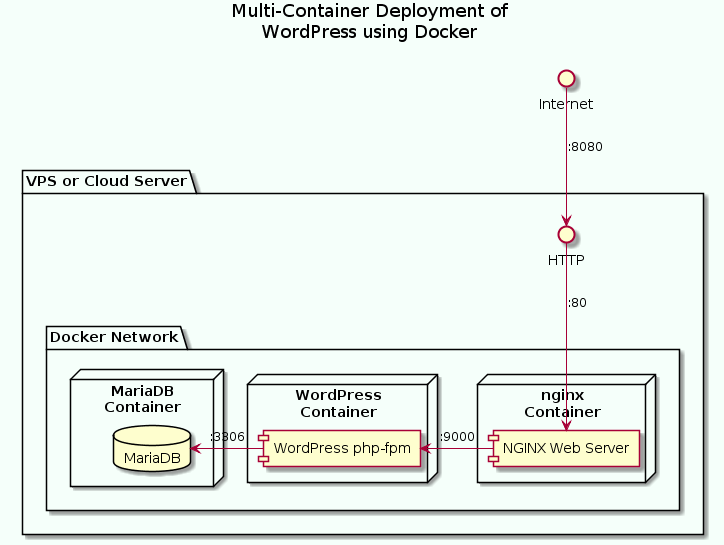
\includegraphics[width=\linewidth]{figures/multi-container.png}
 \caption[Multi-container deployment of WordPress using Docker]{\textit{Evaluation followed multi-container deployment of WordPress using Docker}}
 \label{fig:multi-container}
\end{figure}

\section{Automated Vulnerability Addition}\label{sec:automated}
Evaluating fuzzing processes proved to be a challenging task ~\cite{klees2018Evaluation}. Migrating known vulnerabilities to existing software, to test the fuzzer's capabilities in detecting bugs can be a tedious process ~\cite{bug-reproduction}. For evaluating \pname{}, and other fuzzers for web applications, an \emph{automated bug injection} tool named {\tt Centaur}, inspired by LAVA ~\cite{dolan2016lava} was used for automatically injecting bugs in web applications written in PHP. 

Injecting vulnerabilities in web code was a demanding task, since the necessary tools for analysing \emph{native code} and injecting vulnerabilities (\eg taint-tracking and information-flow frameworks), are not available for web applications. 

To overcome the lack of available tools, {\tt Centaur} uses vulnerability injection methodology to leverage the \emph{instrumentation} infrastructure. The automated bug-injection method can inject hundreds of common vulnerabilities such as Reflected Cross-Site Scripting in reasonable time. 

\section{Evaluation Details}
To evaluate \pname{}'s performance we used two Ubuntu 18.04 LTS Linux machines both possessing a 3.20 GHz quad-core Intel® Xeon® W-2104 Processor and 64 GB of RAM. Targeted web applications consist of (a) an instrumented WordPress 5.5.1 with artificial bugs, (b) a vanilla  WordPress 5.5.1 with artificial bugs, (c) an instrumented Drupal 9.0.6 (d) an instrumented Firefly-III 5.4.6, and (e) an instrumented Mautic 3.0. The term vanilla refers to web-apps in their original form, with no customization or frameworks added to them. 

All artificial bugs were created with the automated vulnerability injection tool mentioned in  Section ~\ref{sec:automated}. Using this methodology, we managed to inject 150 identical Reflected Cross-Site Scripting bugs successfully in both the instrumented and vanilla versions of WordPress. Lastly, the Docker Stack of services described in Section ~\ref{sec:dockerStack} was deployed to run the aforementioned web applications.

For evaluating the performance of \pname{}, the following metrics were used in order of importance:
\begin{itemize}
	\item \emph{Vulnerabilities Detected}: Number of Reflected Cross-Site Scripting bugs reported
	\item \emph{Global Code Coverage}: Accumulated coverage score of the web application's code
	\item \emph{Throughput}: Requests made per second
\end{itemize}

To compare the Vulnerabilities Detected and the Throughput of \pname{} against other black-box fuzzers we used Wfuzz ~\cite{wfuzz}, Burp Suite Professional ~\cite{burp} and OWASP ZAP ~\cite{ owaspzap}. All three of these tools are considered essential in any penetration tester's arsenal as they are included by default in Kali Linux and widely used in Capture The Flag competitions such as GoogleCTF. Other tools; such as {\tt nikto}, {\tt w3af}, {\tt skipfish} and {\tt wapiti} were also used during the evaluation phase but as they were not able to uncover any real or artificially injected bugs we opted not to include them in our final evaluation. The main comparison was made against Wfuzz due to the ease of operation and to extend. The choice of Wfuzz as the main comparison of our tool is further elaborated on in Chapter ~\ref{sec:discussion}.

\section{Evaluated Metrics}

\subsection{Vulnerabilities Detected}
To evaluate how well \pname{} performs in terms of bug detection, we injected 150 artificial  Reflected Cross-site bugs with the methodology we discussed in Section ~\ref{sec:automated} and 4 real Reflected Cross-site Scripting bugs to the instrumented version of WordPress and tested how 3 well-known black-box fuzzers performed in comparison with \pname{}. The real-life RXSS bugs were found from CVE ~\cite{cve} and have the following ids: CVE-2018-7280, CVE-2019-11843, CVE-2020-7104, CVE-2020-7107.

\begin{table}[ht]
\centering
 \begin{tabular}{@{}|l|l|l|l|l|@{}}
 \hline
  \multicolumn{5}{|c|}{\textit{\textbf{Vulnerability Detection}}} \\
 \hline
 \textbf{Tool} & \textbf{Version} & \textbf{Real Bugs} & \textbf{Artificial Bugs} & \textbf{Runtime} \\ 
 \hline\hline
 \pname{} & 1.0.0 & 1 & 30 & 65h  \\ 
 \hline
 Wfuzz & 2.4.5 & 1 & 28 & 65h  \\ 
 \hline
 Burp Suite Professional & 2020.9.2 & 1 & 0 & 7h \\ 
 \hline
 OWASP ZAP  & 2.9.0 & 1 & 0 & 1h  \\
 \hline
 \end{tabular}
 \captionsetup{justification=centering}
 \caption[Vulnerability detection summary]{\textit{Summary of the vulnerability detection evaluation with the findings of 4 fuzzers including \pname{}. The WordPress web-app included 4 RXSS bugs found from CVE and 150 artificial RXSS bugs injected manually}}

 \label{tools_table}
\end{table}

When analysing the specifics of the four real-life RXSS vulnerabilities manually injected, it was realised that CVE-2019-11843 depends on JavaScript code to create its triggering link dynamically in the form of an {\tt anchor} element. Also, for the vulnerability CVE-2018-7280 to trigger it is compulsory for the XSS payload to be injected inside a specific JSON object at one of the vulnerable {\tt form}'s parameters. The other three depend on JavaScript code to dynamically append the vulnerable POST parameter upon {\tt form} submission. 

The real RXSS bug that all four tools were able to detect was CVE-2020-7107. This bug was related to the Ultimate FAQ plugin for WordPress. More specifically, the HTML code generated by the FAQ shortcode (WordPress-specific code that simplifies complex commands) did not sanitise the Display-FAQ GET parameter, leading to the unauthenticated RXSS issue on pages where such shortcode is used. This vulnerability was fixed in a later version (1.8.30) of the plugin by sanitizing the GET parameter with the {\tt intval()} function. 

As Table ~\ref{tools_table} shows, all tools involved in the evaluation only managed to find one real-life RXSS bug. This is because none of them employs complex enough JavaScript code analysis nor do they run a request's client-side code to uncover these dynamic links and parameters.

It is important to note that vulnerability scanners such as Burp Suite Professional provide a Proxy service that can intercept web browsing traffic so that requests created dynamically by client-side code can be fuzzed as well. Nevertheless, we chose to avoid these features since \pname{} currently lacks this functionality and thus, it would be an unfair comparison.

As clearly observed in Table ~\ref{tools_table}, the results of all fuzzers for real-life bugs are disappointing. For this reason, we further evaluated the fuzzing tools on how well they perform with artificially injected bugs (Section ~\ref{sec:automated}). Because OWASP ZAP and Burp Suite Professional do not generate the required format of injection payloads unless advanced features and modifications are in place, they were unable to detect any of the artificially injected bugs. Using their advanced features requires extensive research and training. As the learning curve is steep, we decided to only customise Wfuzz.

For a fair comparison of the vulnerability detecting capabilities of \pname{} and Wfuzz, some modifications were made to the latter since originally the tool was meant to be a simple brute-forcer and not a black-box fuzzer. An independent crawling process was added at the start to infer the control flow of the web application. 

The findings are stored and fed to Wfuzz as a list of fuzz targets. Utilising the Python module version of Wfuzz, a Python script was created that fuzzes the list of links found by the \emph{crawler}, indefinitely. Payloads used during the fuzzing process are customised to resemble the mutated payloads that \pname{} uses. They consist of random strings, HTML syntax tokens, and random numbers all concatenated with the same XSS payloads that webFuzz uses from its corpus described in Chapter ~\ref{sec:architecture}.

\begin{figure}[!htb]
  \centering 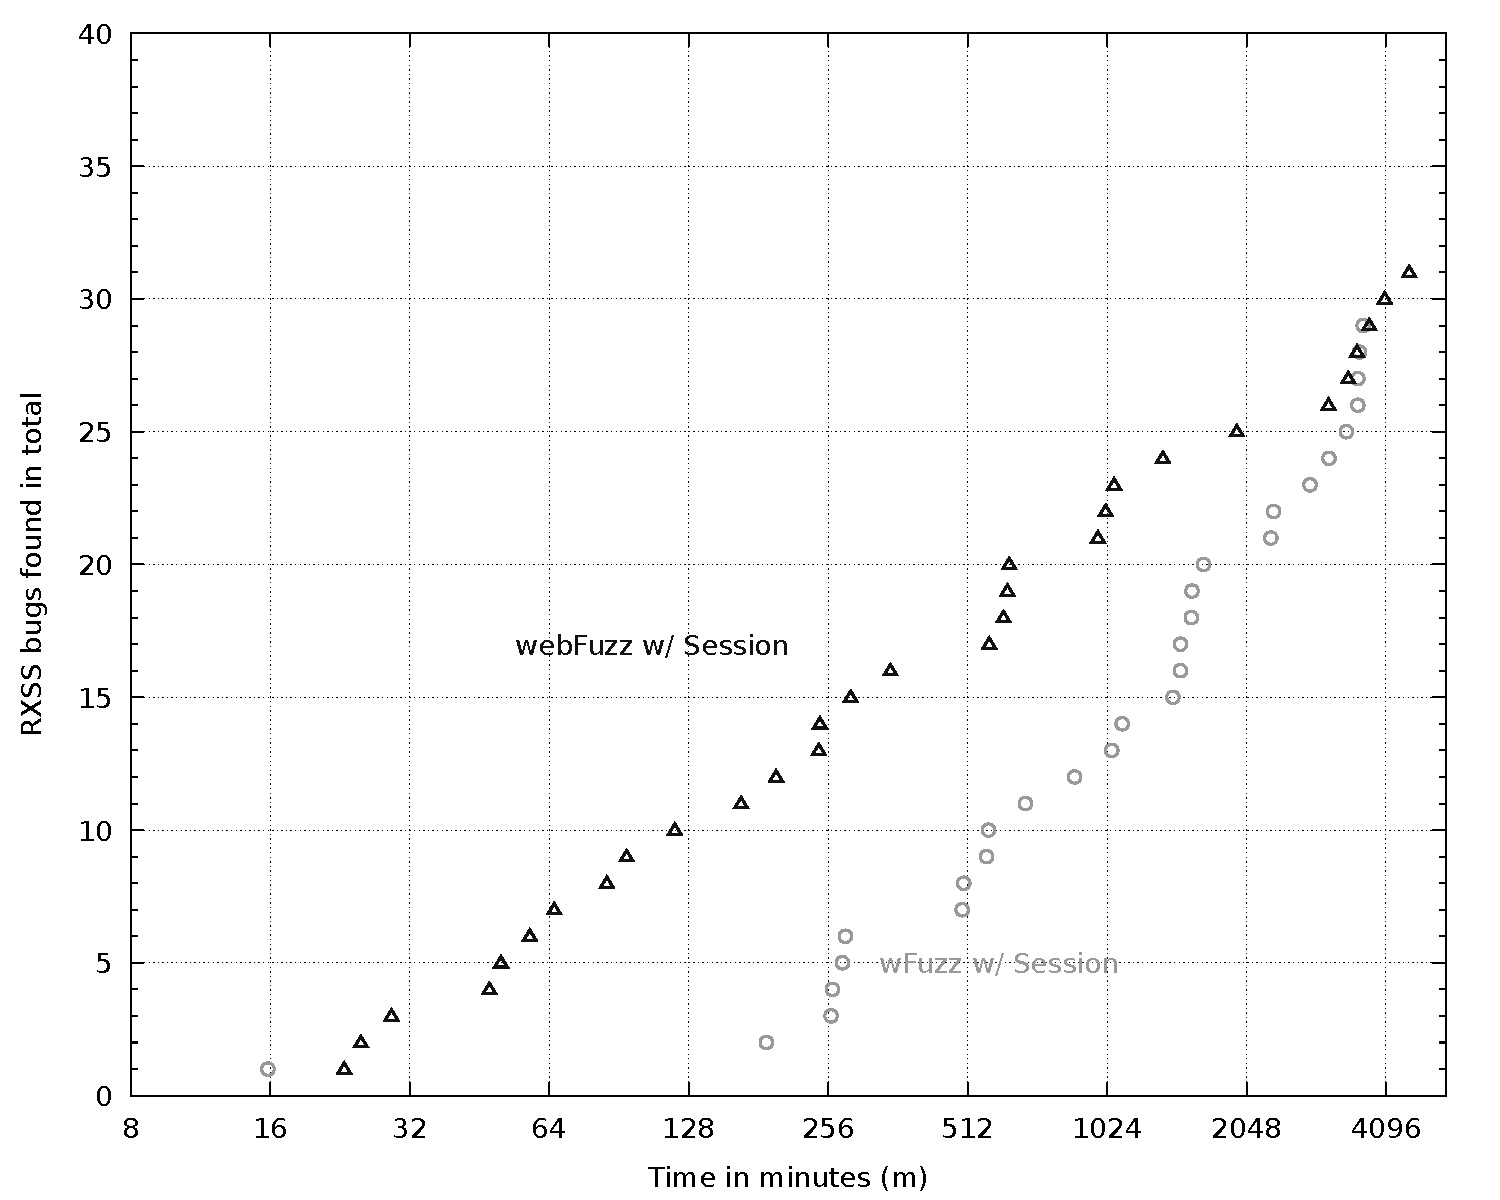
\includegraphics[width=\linewidth]{figures/plot_bugs.pdf}
  \captionsetup{justification=centering}
  \caption[Number of artificial XSS bugs uncovered by \pname{} and Wfuzz]{\textit{Artificial Reflected Cross-Site Scripting bugs detected over time by \pname{} and Wfuzz. \pname{} manages to uncover more bugs quicker during the fuzzing process}} 
  \label{fig:plot_rxss}
\end{figure}

The results of our 65-hour experiment, comparing Wfuzz and \pname{} in terms of artificial RXSS bugs found is seen in Figure ~\ref{fig:plot_rxss}. Although \pname{} leads throughout the entire experiment, the difference decreased until the end when it became marginal. \pname{} uncovered 30 artificial bugs, two more than the Wfuzz's 28.

By taking advantage of the \emph{instrumentation feedback loop}, \pname{} detected the artificial bugs faster than Wfuzz's brute force approach. Whenever a digit of a \emph{magic number}, situated in a vulnerable payload, is guessed correctly, our fuzzing tool will detect this change and prioritize the request that causes it. 

With this method, finding a \emph{magic number} is done incrementally - one correct digit at a time - which is much faster than guessing the whole number at once like Wfuzz does. As a real-world analogy, each digit of the \emph{magic number} can represent one correct mutation that brings us closer to the vulnerable basic block. A reason for the gradual decrease of webFuzz's detection performance lies in its growing request queue size. WordPress is composed of approximately half a million LoC, with 48,040 basic blocks instrumented in total.

\subsection{Global Code Coverage}
Utilizing the \emph{instrumentation} feedback, \pname{} has calculated the global code coverage for WordPress, Drupal, Firefly-III and Mautic. For these four PHP open-sourced projects, we decided to test only the authenticated session scenarios as the unauthenticated session would prevent us from  accessing various links such as the administrative dashboard related links. In Figure ~\ref{fig:plot_coverage}, we see how the metric changed over time in the four authenticated session scenarios.

\begin{figure}[!htb]
  \centering 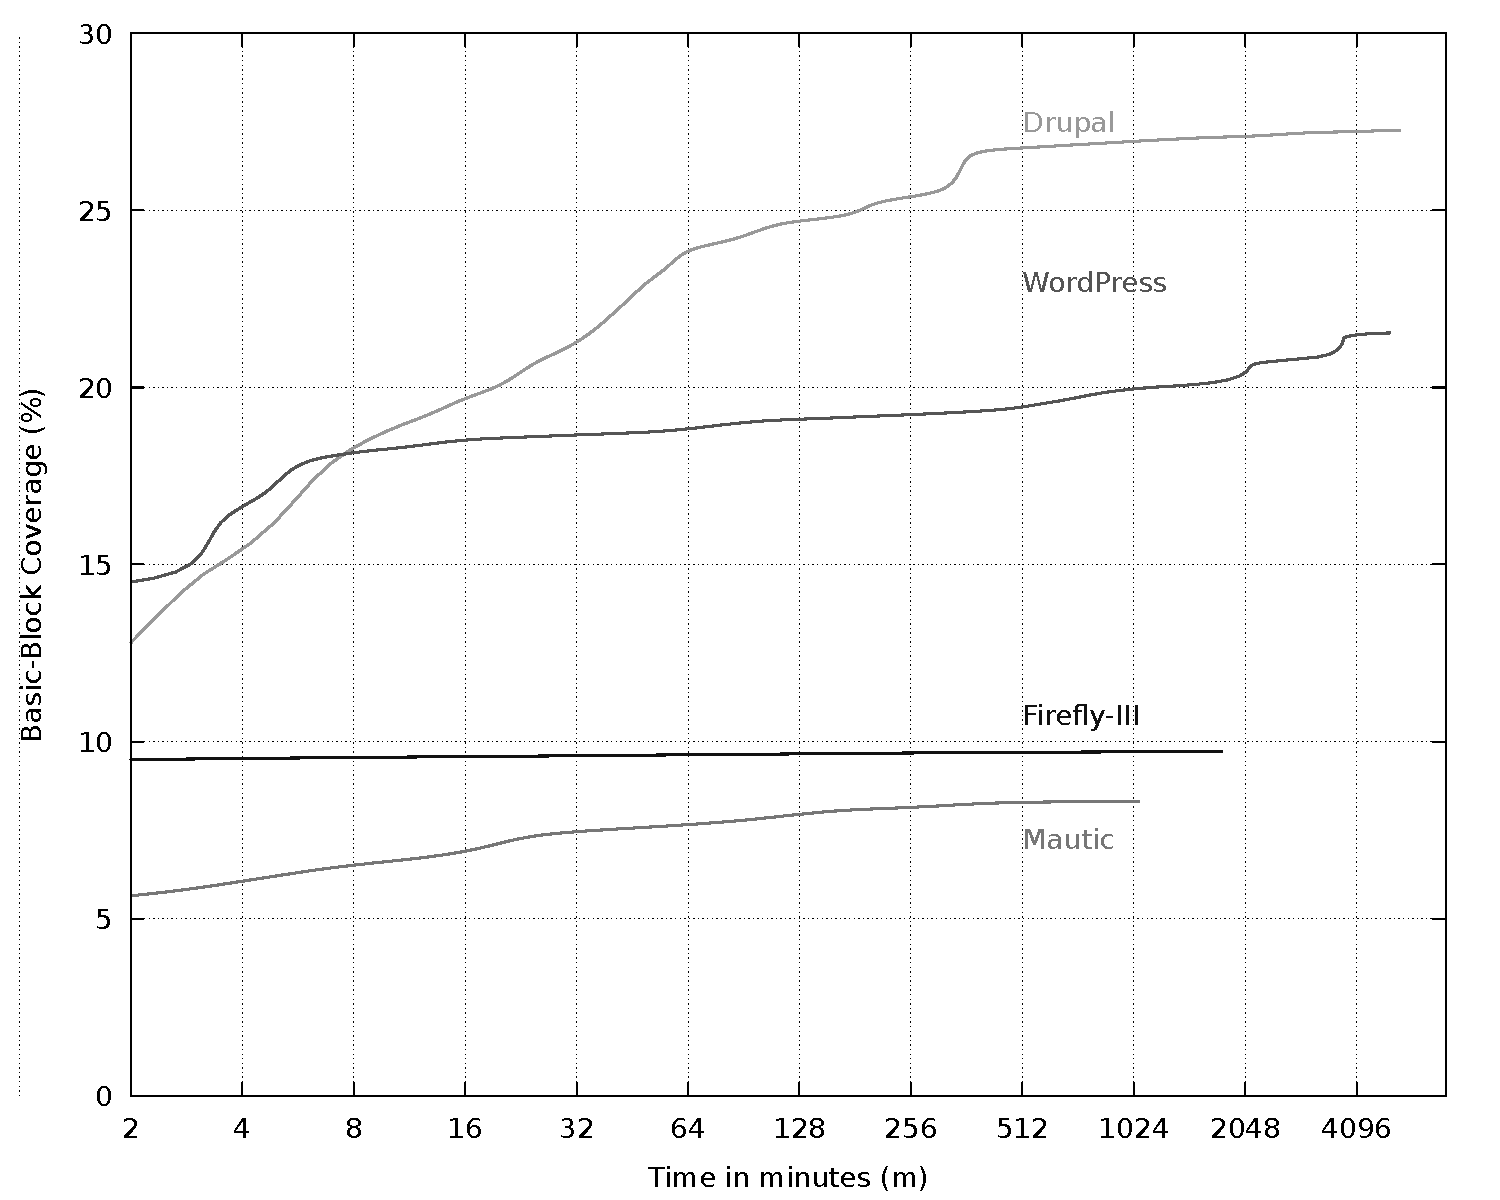
\includegraphics[width=\linewidth]{figures/plot_coverage.pdf}
  \captionsetup{justification=centering}
  \caption[Accumulated global code coverage using \pname{}]{\textit{Four different execution scenarios and the accumulated code coverage gained over time. Exponential increases at the start of the experiment are due to initial exploration of the target web application's site map by the crawler}} 
  \label{fig:plot_coverage}
\end{figure}

\begin{table}[h]
\centering
 \begin{tabular}{@{}|l|l|l|@{}}
 \hline
 \multicolumn{3}{|c|}{\textit{\textbf{Code coverage achieved with \pname{} }}} \\
 \hline
 \textbf{Fuzz target} & \textbf{Run time (minutes / days)} & \textbf{Code coverage (\%)} \\ 
 \hline\hline
 Drupal & 6000 / 4.2 & 27.3 \\ 
 \hline
 WordPress & 6000 / 4.2 & 21.5 \\ 
 \hline
 Firefly-III & 1900 / 1.3 & 9.7 \\ 
 \hline
 Mautic & 1024 / 0.7 & 8.3 \\ 
 \hline
 \end{tabular}
 \captionsetup{justification=centering}
 \caption[Code coverage achieved by \pname{}]{\textit{Code coverage achieved by \pname{} when fuzzing four open-source web applications}}

 \label{coverage_table}
\end{table}

Our experiment showed the two main web applications of our evaluation, Drupal and WordPress accrued the most basic-block coverage with \emph{27.3\%} and \emph{21.5\%} respectively. Firefly-III was stopped after 1.3 days as the coverage remained static at \emph{9.7\%} during the entire time. In the case of the fourth fuzz target Mautic, we agreed to terminate this test early (0.7 days) as the throughput was arduously slow in reaching the desired level of code coverage within a reasonable time limit (see Table ~\ref{coverage_table}). 

More importantly, the code coverage achieved by \pname{} in both the Drupal and WordPress scenarios indicate a steady rise in the global code coverage even after 6000 minutes of execution time. An encouraging signal that the mutation functions used are effective enough to trigger new code paths, even after the crawling process has finished. 
 
\begin{figure}[!htb]
  \centering 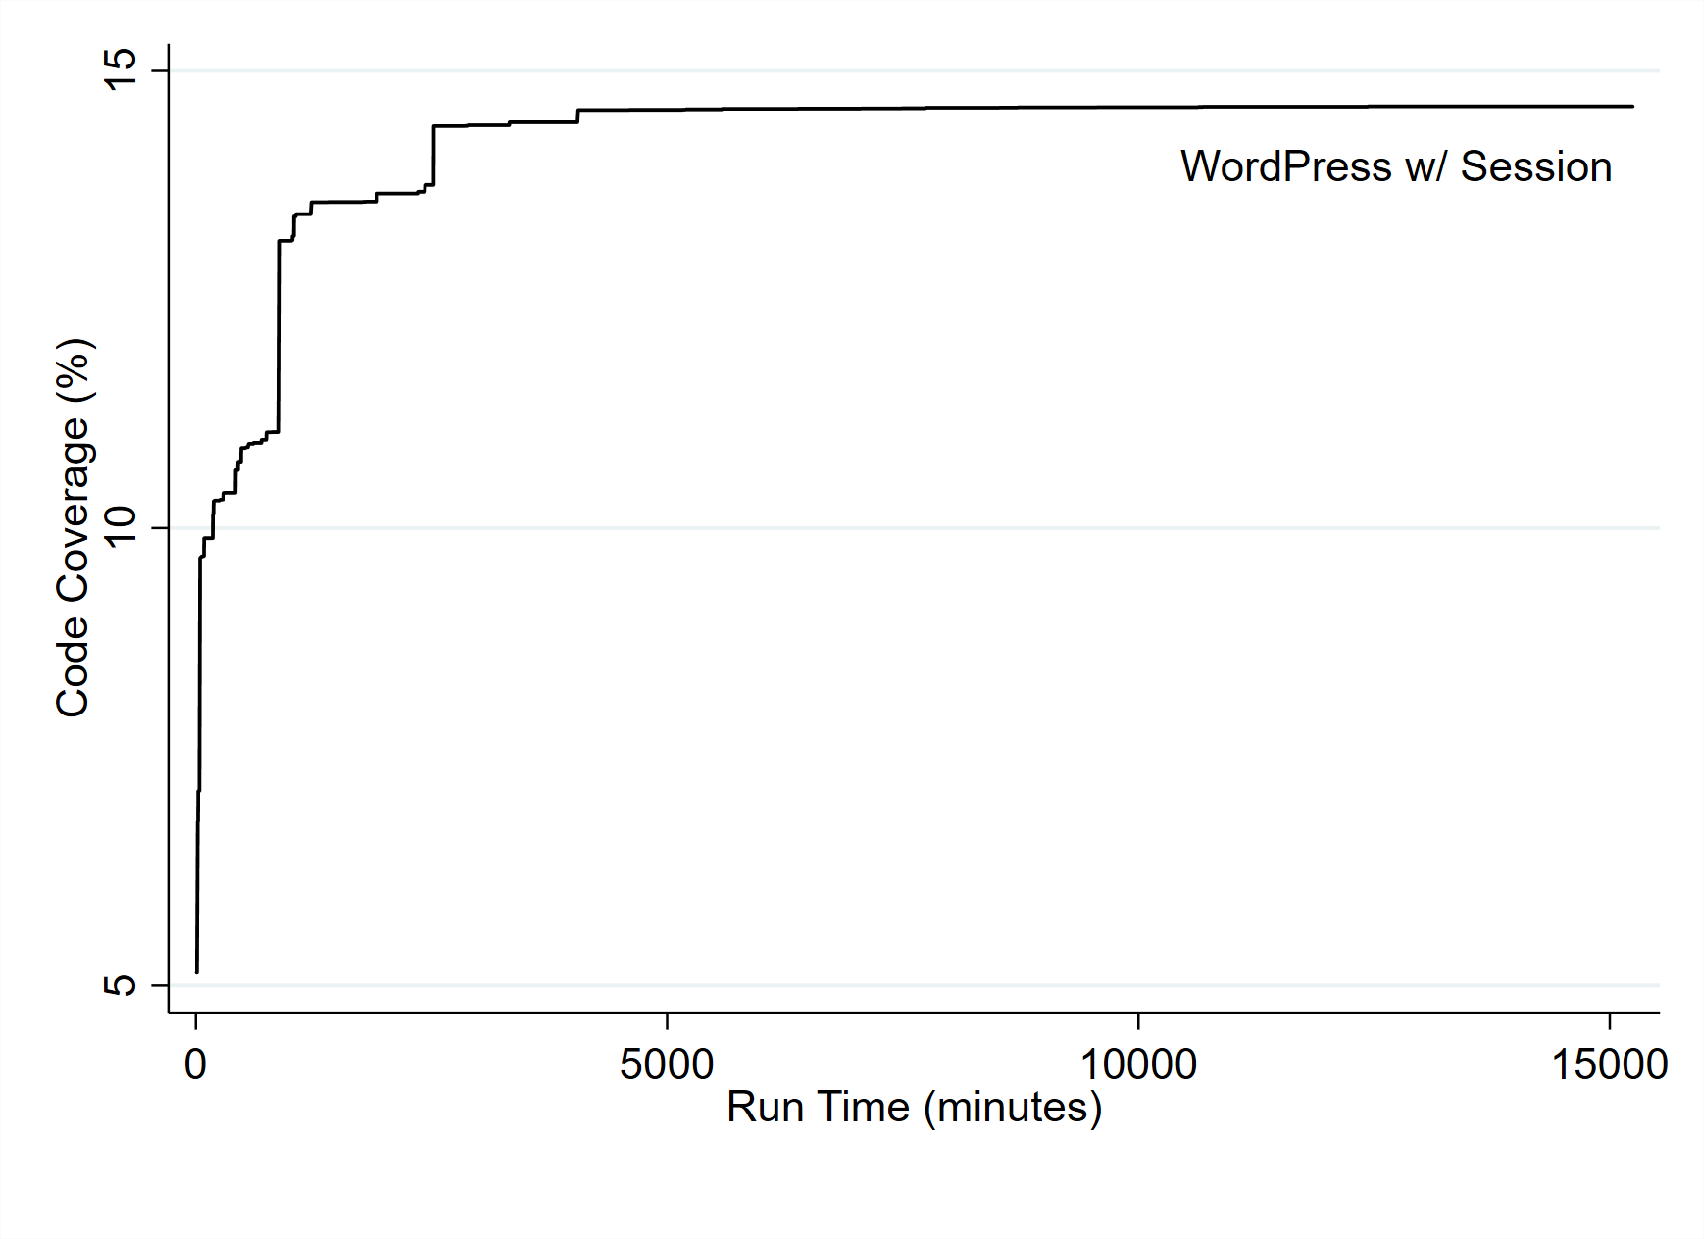
\includegraphics[width=\linewidth]{figures/plot_coverage2.pdf}
  \captionsetup{justification=centering} 
  \caption[Accumulated global code coverage using Wfuzz]{\textit{Code coverage achieved by Wfuzz over time when fuzzing WordPress using an authenticated session. After running for approximately 5000 minutes (3.5 days) the code coverage remained stagnant at 14.6\% for the rest of the experiment}}
  \label{fig:plot_coverage2}
\end{figure}

In Figure ~\ref{fig:plot_coverage2} we can see the Global Code Coverage achieved by the black-box fuzzer Wfuzz when fuzzing WordPress using an authenticated session. The peak of this experiment was reached in roughly \emph{3.5} days (5000 minutes) when code coverage of \emph{14.613\%} was reached. This experiment was solely to check how well a black-box fuzzer performs in terms of code coverage against a grey-box fuzzer, like \pname{}, that leverages \emph{instrumentation} feedback. 

When looking at Figures ~\ref{fig:plot_coverage} and ~\ref{fig:plot_coverage2}, we can safely surmise that the \emph{instrumentation} feedback provides \pname{} with the edge needed to surpass the performance of Wfuzz. More precisely, when both were fuzzing WordPress with an authenticated session, \pname{} managed to get almost \emph{1.5} times higher code coverage than Wfuzz. Wfuzz was left running for a much longer time (10.4 days) than \pname{} with no luck since it stayed stagnant on the score it achieved after 3.5 days at \emph{14.613\%}.

\subsection{Throughput}

\begin{figure}[!htb]
  \centering 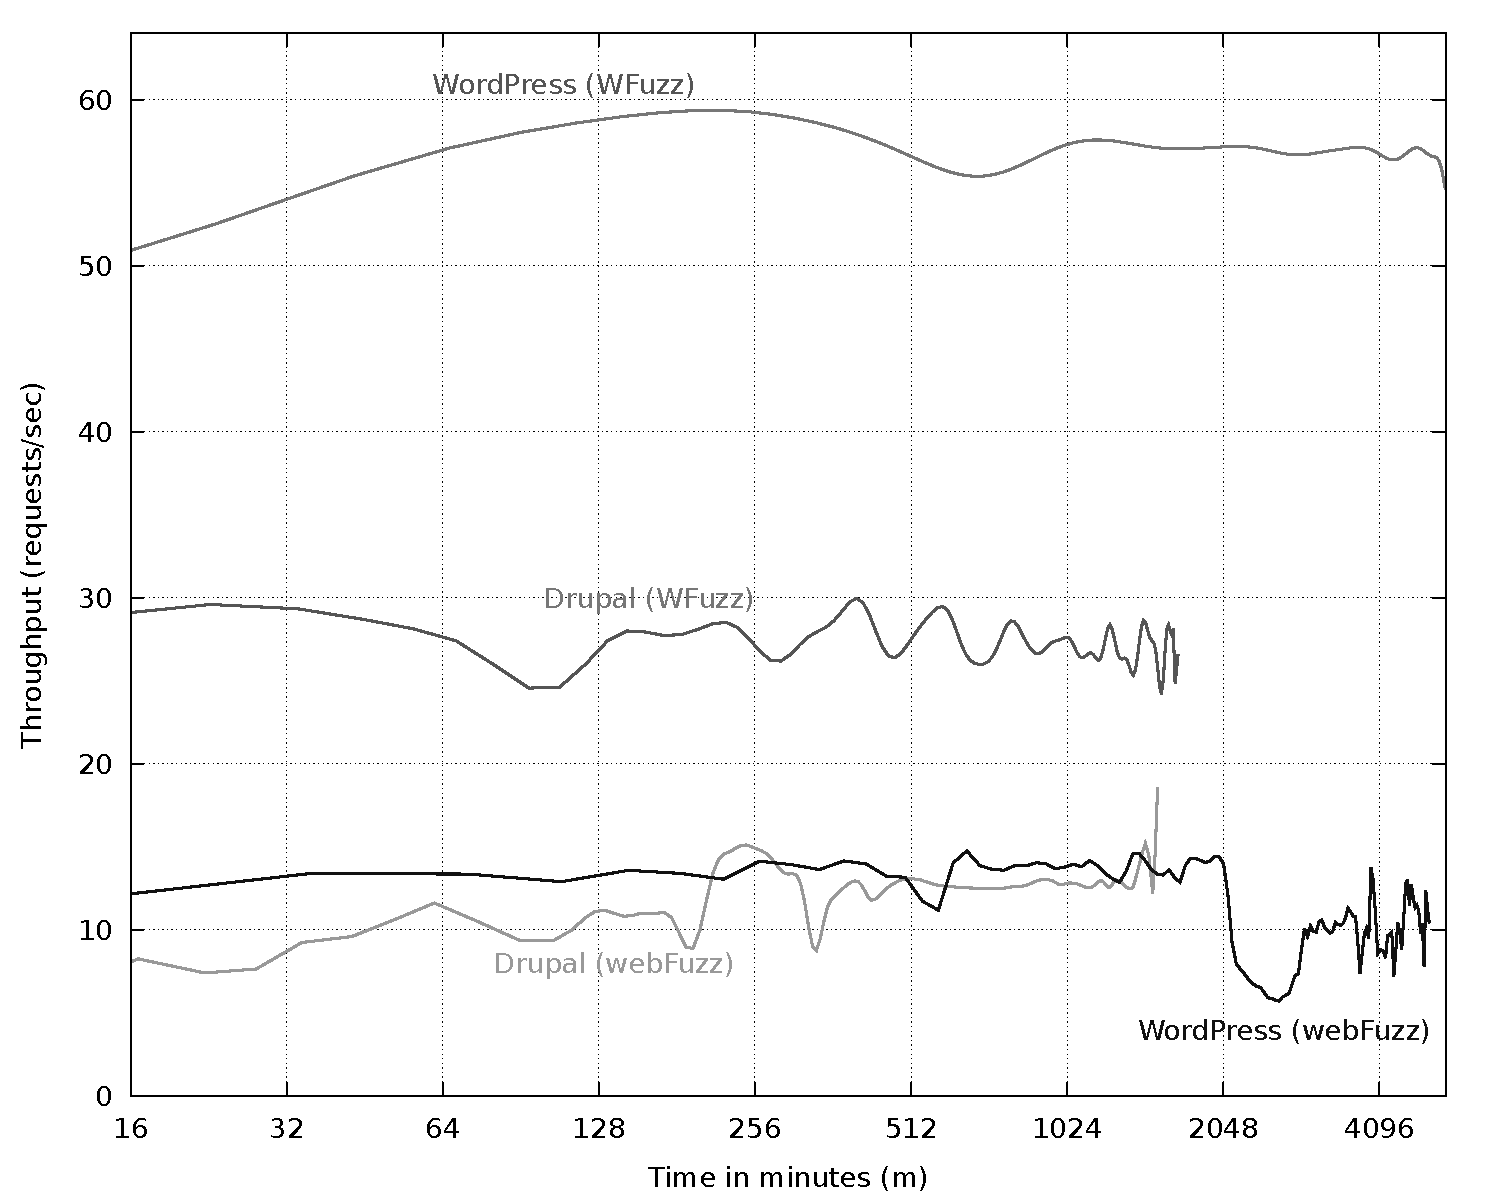
\includegraphics[width=\linewidth]{figures/plot_throughput.pdf}
  \captionsetup{justification=centering}  
  \caption[Throughput of \pname{} and Wfuzz when fuzzing Drupal and WordPress]{\textit{Requests made per second over time for three different scenarios. Both \pname{} and Wfuzz are evaluated on Drupal and WordPress. Wfuzz takes the lead with a difference}} 
  \label{fig:plot_throughput}
\end{figure}

One reason for the effectiveness of fuzzers in uncovering vulnerabilities is their capability to test vast amounts of inputs per second. The overhead caused by \emph{instrumentation} must not severely degrade the web application's response time and the fuzzer's processing time for each request is kept as brief as possible.

As observed in Figure ~\ref{fig:plot_throughput}, the black-box version of Wfuzz has about \emph{3} times higher throughput than \pname{} in the case of Drupal and \emph{4.5} times in WordPress. This is plausible as the overhead added from \emph{instrumentation} roughly doubles the page response time for WordPress, and due to webFuzz's increased statefulness in tracking, analysing and ranking all the requests, it increases the per-request processing time.

After 2,048 minutes in WordPress using \pname{} with an authenticated session established, the throughput plummets for a lengthy period. This implies that the fuzzer was stuck on fuzzing particular links that have lofty response times. The fact our fuzzer keeps on fuzing these links mean they have a high coverage score and mutating them is effective enough to trigger new code paths.

Looking at Figure ~\ref{fig:plot_throughput}, we can state with confidence that much needs to be done to improve the throughput of \pname{}, since it is nowhere near that of native application fuzzers such as AFL and EFS nor is it comparable to black-box web fuzzers such as Wfuzz. That was no more than expected as native applications have no need to address overhead from sending requests over a network. Needless to say, the necessary improvements are discussed in the next chapter.
\chapter{Discussion}
\label{sec:discussion}
\minitoc
\vspace*{1cm}

In the discussion chapter, the limitations faced - such as a lack of fuzzers to compare with - during the development of \pname{} are outlined in detail. There are also deliberations on future plans and what is being considered to upgrade our fuzzing tool.

\section{Limitations}
During the development of \pname{} we faced various obstacles that must be addressed to produce a more productive tool.

Our first major obstacle was the choice of Wfuzz as the main fuzzer to compare \pname{} with. After extensive research, it became apparent there are fewer black-box fuzzers available today as there were a decade ago. Many older and renowned black-box fuzzers mentioned in various websites and published papers ~\cite{doupe2010johnny, bau2010state, duchene2014kameleonfuzz} have either ceased to exist or are no longer developed and maintained. 

During our research, we discovered that Wfuzz is the only tool that can be imported as a module in Python, thereby extending its functionality. Although Wfuzz is classified as a 'brute-forcer', by providing the aforementioned functionality we can add code and make it operate as a black-box fuzzer. This enabled us to make a reasonable comparison with our fuzzing tool. Wfuzz was easier to use as it did not require time-consuming research and extra training. This could not be achieved with Burp Suite Professional or OWASP ZAP.

Additionally, during the evaluation phase, more evidence could be submitted to further explore the potential of \pname{} in detecting vulnerabilities. For instance, the tool can be evaluated on more open-source projects written in PHP and tackle other complex real-world XSS vulnerabilities, that reflect real-world scenarios. A case in point, CVE is a good source of finding publicly-known XSS vulnerabilities. A recent paper by Backes et al. ~\cite{efficient2017} proposes ideas on such large-scale analysis of web application code to find real-world XSS bugs. We will use this as a reference point going forward. 

For now, webFuzz's vulnerabilities detection suite is limited to Reflected and Stored Cross-Site Scripting. DOMbased XSS vulnerabilities that rely on the browser's JavaScript runtime context, are beyond the fuzzer's scope. These types of attacks require no interaction with
the server, and succeed when the JS code does not sanitize the user input before rendering it unfiltered (\eg using the {\tt innerHTML} property). For detecting these vulnerabilities, we would need to render the HTML and run the JavaScript code of each request. This would severely degrade the fuzzer's throughput, that is why this type of detection was not included for the initial version of \pname{}.  Unfortunately, by excluding JavaScript, due to a time deficit, many potential XSS vulnerabilities will go undetected.

\section{Future Work}
Our work is not yet done. Despite our initial accomplishments there is much we need to do to take this promising fuzzing tool to another, higher, level. Undoubtedly, improvements need to be made to ensure it is an effective and trustworthy tool. Below are some ideas on future progress.

There are future plans to include more functionalities in our tool kit to weed out other critical web-app vulnerabilities through our detection suite, so it can provide wider security protection that goes beyond Cross-Site Scripting. 

Such core vulnerabilities can be found at OWASP Top 10 ~\cite{owasp2017} the most common form of bug in web applications is Injection and Broken Authentication. Injection flaws, such as SQL and NoSQL, occur when untrusted data is sent to an interpreter or database as part of a query. For this specific vulnerability, various known payloads have already been collected ~\cite{seclist} - the same way as the XSS payloads are - and stored in the repository waiting for the respective functionality to be added to \pname{}.

There are also plans to implement a more efficient string-matching algorithm that will decrease the number of false positives we can currently record. This can be achieved by taking into consideration the location of the payload in the HTML document. These types of improvement will enable us to detect Cross-Site Scripting vulnerabilities that are triggered due to HTML attributes such as {\tt onchange } and {\tt onclick}, and not because of the HTML's <script>.

As we mentioned in the limitations, previous research used techniques such as analysis of JavaScript code or Selenium-based crawlers to include the JavaScript-generated request URLs in their analysis. We could adopt similar approaches since we are currently missing many bugs by excluding JavaScript. Moreover, to improve our evaluation we may adopt similar approaches that Backes et al. did  ~\cite{efficient2017} where they propose a way to build code property graphs for 1,854 popular open-source PHP projects on GitHub, storing them in a graph database and detect vulnerabilities through flow-finding traversals.

One idea on improving our fuzzer is that certain core functions of the
fuzzer might eventually be ported to faster languages; such as C and Java, that can substantially enhance speed performance and reduce memory consumption. Besides, a per link time-out will be introduced, to avoid I/O heavy web pages from stalling the fuzzing process. Initial work has also be done with netmap  ~\cite{rizzo2011Netmap}, a framework that modifies kernel modules to effectively bypass the Operating System's network stack, which often creates a bottleneck between client and server communication, to achieve a high-speed packet I/O.

Also to be included, are more Python modules to improve the overall performance of \pname{}. Since our fuzzer requires a lot of file I/O to do its logging work, the {\tt mmap } module can be utilised by using lower-level operating system APIs to load a file directly into the computer memory and read/write files as if they were one large string or array ~\cite{mmap}. 

Another module that could boost the performance of \pname{} is aiomultiprocess ~\cite{aiomultiprocess}. As we briefly mentioned in Chapter ~\ref{sec:background}, AsyncIO is limited to the speed of GIL, and multiprocessing entails spreading tasks over a computer's cores. By combining the two, we can overcome these obstacles to truly achieve 'parallelism' in Python. Achieving 'parallelism' would be a beneficial outcome as today's PCs/laptops have processing units with multiple cores.

Having said this, ideas of optimization are one thing, putting them into practice is an entirely different matter. Every step has to be properly assessed and examined scientifically before they can be added to our tool.

\textit{"Premature optimization is the root of all evil (or at least most of it) in programming," said Donald Knuth - the father of algorithms analysis.}
\chapter{Related Work}
\label{sec:relatedwork}
\minitoc
\vspace*{1cm}

In this chapter any relevant work done in the past year at research level to the field of fuzzing is stated here.

\section{Generic Fuzzing}
Fuzzing has been perceived through several techniques and algorithms over the years. Firstly, we have the black-box fuzzers ~\cite{householder2012probability,sparks2007automated,woo2013scheduling} which are unaware of the fuzz target's internals and thus are trying to trigger vulnerabilities by randomly generating the inputs. While the black-box fuzzers category might not be as performant as others, they offer
the advantage of compatibility with any program ~\cite{osterlund2020parmesan,rawat2017vuzzer}. The other two categories are white- and grey-box fuzzers. These two leverage instrumentation to obtain feedback concerning the inputs' precision in discovering unseen paths. 

It is proven that the feedback is vital for a fuzzer's performance since it can be used to steer the fuzzer towards exploring new code paths, resulting in a better code coverage also known as
coverage-based fuzzers. Otherwise, we have the directed based fuzzers that use feedback to direct the fuzzer towards particular execution paths ~\cite{godefroid2005dart}.

A renowned fuzzer that is classified as coverage-based is AFL ~\cite{zalewski2015american}. AFL is a state-of-the-art grey-box fuzzer which is deemed the foundation for the majority of the recent proposed works. However, AFL fails to intelligently generate inputs to explore deep paths in programs that are hidden behind checksums or magic number \emph{if} statements.

Having this in mind, recent research work makes use of symbolic and concolic execution to enhance the input generation procedure by extracting valuable information about the program. Some examples consist of DRILLER ~\cite{stephens2016driller}, DART ~\cite{godefroid2005dart} and SAGE ~\cite{godefroid2012sage}. 

In spite of all these efforts to improve the fuzzing process with the use of symbolic/concolic execution based fuzzers, it has been noticed that this type of fuzzers suffer from scalability problems because when fuzzing sizeable targets, we notice the problem of state explosion ~\cite{Clarke2012}. This problem is observed when the number of state variables in the system increases, the size of the system state space grows exponentially making it impossible to explore the entire state space with limited resources of time and memory.

Consequently, some other research proposals try to accomplish what symbolic/concolic execution based fuzzers offer with a less expensive approach. One example is REDQUEEN ~\cite{aschermann2019redqueen} that utilizes the input-to-state correspondence in order to infer the values that would be later used and try control them. Another such example is VUzzer ~\cite{rawat2017vuzzer}, an application-aware evolutionary fuzzer that leverages control and data-flow features using static and dynamics analysis to infer fundamental properties of the fuzz target.

\section{Web Applications Fuzzing}
Even Though a huge effort have been given to build fuzzers with the aim to weed out vulnerabilities in native code, little attention has been given to web applications bugs. Tools currently available that target web application vulnerabilities behave predominantly in a black-box fashion, therefore, they are unable to uncover vulnerabilities that are embedded deep into the web application ~\cite{bau2010state, doupe2010johnny}.
 
Such as SecuBat ~\cite{kals2006secubat}, a web vulnerability scanner that uses a black-box approach to detect SQL injection(SQLi) and Cross-Site Scripting(XSS) vulnerabilities. Another example is KameleonFuzz ~\cite{duchene2014kameleonfuzz}, a black-box fuzzer for web vulnerabilities targeting XSS susceptibilities.

There have been attempts to overcome the shortcomings of black-box techniques. Doupé et al. ~\cite{doupe2012enemy} proposed a way to navigate through a web application's states to discover whether an input is interesting by noticing the changes of the output. 

As an alternative, there is the white-box approach to consider with access to the web application's source code. Kieyzun et al. ~\cite{kieyzun2009automatic} used a technique exploiting information about the code to automatically generate inputs that target SQLi and XSS vulnerabilities. 

Moreover, Artzi et al. ~\cite{artzi2010finding} developed another tool for discovering web
application vulnerabilities by collecting information about the target extracted through concrete and symbolic execution.

White-box methods outperform black-box approaches by having access to the source code of the target being fuzzed. However, black-box processes are more scalable when the source code is not 
available. 

To conclude, web vulnerability scanners are also realized through static analysis tools. Prime examples are Pixy ~\cite{jovanovic2006pixy} which uses static analysis at the source code
level to detect vulnerable code. 

Another tool combining static and dynamic analysis is Saner ~\cite{balzarotti2008saner} which tries to identify any sanitization processes that do not work as expected to, resulting in allowing attackers to introduce exploits.

Contrary to the above research work for identifying web vulnerabilities, our technique adopts the
grey-box approach. \pname{} instruments the fuzz target to receive feedback on whether a generated input is interesting. These inputs are used to generate other test cases that will hopefully result in wider code coverage that could possibly trigger more vulnerabilities. Unlike other fuzzers mentioned who generate their own XSS payloads ~\cite{duchene2014kameleonfuzz}, our tool's  main objective is finding trigger points on the target web application and supplying them with known XSS payloads.
\chapter{Conclusion}
\label{sec:conclusion}
\minitoc
\vspace*{1cm}

% NEW SECTION
\section{Conclusion}

% NEW SECTION
\section{Future Work}
As Donald Knuth has said, “Premature optimization is the root of all evil (or at least most of it) in programming.”

% bibliography
\bibliographystyle{abbrv}
\balance
\bibliography{./bibliography/thesis}
\addcontentsline{toc}{chapter}{Bibliography}

% Appendices
\begin{appendices}
	\titlespacing*{\chapter}{0pt}{0pt}{0pt}
	\chapter{}
\renewcommand{\thepage}{\thechapter-\arabic{page}}
\setcounter{page}{1}
\label{sec:appendixa}

\begin{framed}
\lstinputlisting[frame=single, language=Python, caption={\textit{Docker-compose file used during the deployment of WordPress}}, numberstyle=\color{gray}, numbersep=5pt, label={lst:dependencies}]{./appendices/docker-compose.yaml}
\end{framed}
	\chapter{}
\renewcommand{\thepage}{\thechapter-\arabic{page}}
\setcounter{page}{1}
\label{sec:appendixb}

\begin{framed}
\lstinputlisting[frame=single, language=PHP, caption=\textit{{Modules needed to be installed so webFuzz can execute smoothly}}, numberstyle=\color{gray}, numbersep=5pt, label={lst:python_dependencies}]{./appendices/requirements.txt}
\end{framed}
	\let\clearpage\relax
\end{appendices}
% that's all
\end{document}
